\documentclass[11pt]{article}
\usepackage[a4paper,margin=2.5cm]{geometry}
\usepackage{amsmath,amssymb}
\usepackage{graphicx}
\usepackage{booktabs}
\usepackage{float}
\usepackage{makecell}
\usepackage{array}
\usepackage[numbers,sort&compress]{natbib}
\usepackage[hidelinks]{hyperref}
\usepackage{url}
\newcommand{\JPLtestN}{8,795}
\newcommand{\CALtestN}{4,828}
\newcommand{\ErrorSentence}{Across the six training windows, the median claimed driver stayed 0.47--0.53\,h longer than declared at JPL and 0.60--0.95\,h longer at Caltech, yet the errors are wide: over the whole period the 10th and 90th percentiles of $\Delta d$ are -2.6 and 5.0\,h at JPL and -1.8 and 6.5\,h at Caltech, and 35\% (JPL) and 31\% (Caltech) of claimed sessions ended before the declared time. Declared energy is biased upwards: the median ratio $\rho$ is 0.61--0.65 at JPL and 0.52--0.57 at Caltech, and 89\% and 98\% of claimed sessions received less energy than requested, consistent with the unreliability of user inputs reported in \cite{Lee2019ACNData}.}

\renewcommand{\thetable}{S\arabic{table}}
\renewcommand{\thefigure}{S\arabic{figure}}
\renewcommand{\thesection}{S\arabic{section}}
\setlength{\emergencystretch}{3em}

\title{Supplementary Material for\\[4pt]
\large Realising grid flexibility from workplace electric vehicle charging under imperfect information and tariff signals}
\author{Mansour Almuwallad\\ \small Department of Management Science, Yanbu Industrial College,\\ \small Royal Commission for Jubail and Yanbu, Yanbu 45130, Saudi Arabia\\ \small almuwalladm@rcjy.edu.sa}
\date{}

\begin{document}
\maketitle

\noindent This document contains supporting tables and figures referred to in the main article as Tables S1--S7 and Figs.~S1--S5. Section, table and figure numbers without the prefix S refer to the main article. All values are computed by the released code and are reproducible from the public repository \cite{ThisStudyRepo}.

\section{Data}
The filtering flow of the 2019 sessions is given in Table~\ref{tab:flow}. Daily delivered energy and the weekday distributions of arrival and departure times are shown in Fig.~\ref{supp:data}. JPL access is restricted to employees, whereas the Caltech garage is open to the public (Section~3.1).

\begin{table}[H]
\centering
\caption{Session filtering flow.}
\label{tab:flow}
\footnotesize
\setlength{\tabcolsep}{1.5pt}
\begin{tabular*}{\textwidth}{@{\extracolsep{\fill}}lp{0.68\textwidth}r@{}}
\hline
Site & Step & Sessions \\
\hline
JPL & raw & 11,830 \\
JPL & drop duplicate session ID & 11,830 \\
JPL & has arrival, departure, kWh & 11,830 \\
JPL & kWh $\geq$ 0.5 & 11,830 \\
JPL & 0.25 h $\leq$ duration $\leq$ 48.0 h & 11,823 \\
JPL & done within [arrival, departure] & 11,823 \\
JPL & implied avg power $\leq$ 20.0 kW (drops DC fast charging) & 11,823 \\
JPL & claimed (usable declaration) & 11,442 \\
JPL & declaration present but invalid $\rightarrow$ treated as unclaimed & 0 \\
JPL & declaration edited after plug-in (first input used) & 0 \\
\hline
Caltech & raw & 6,704 \\
Caltech & drop duplicate session ID & 6,704 \\
Caltech & has arrival, departure, kWh & 6,704 \\
Caltech & kWh $\geq$ 0.5 & 6,704 \\
Caltech & 0.25 h $\leq$ duration $\leq$ 48.0 h & 6,659 \\
Caltech & done within [arrival, departure] & 6,659 \\
Caltech & implied avg power $\leq$ 20.0 kW (drops DC fast charging) & 6,659 \\
Caltech & claimed (usable declaration) & 5,616 \\
Caltech & declaration present but invalid $\rightarrow$ treated as unclaimed & 0 \\
Caltech & declaration edited after plug-in (first input used) & 0 \\
\hline
\end{tabular*}
\end{table}


\begin{figure}[H]
\centering
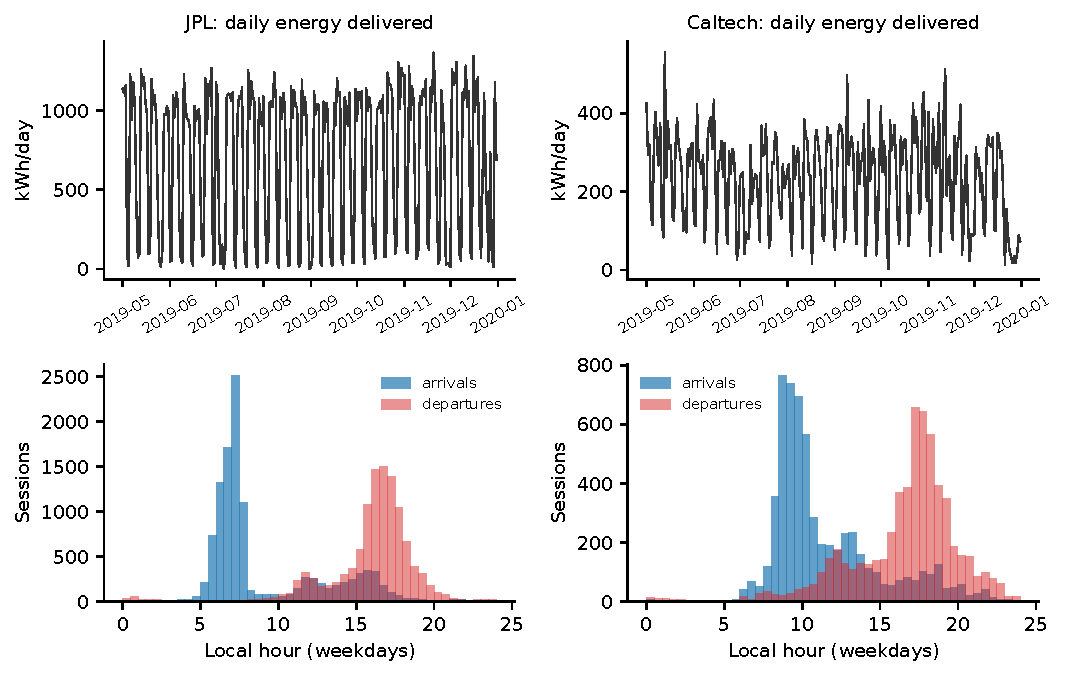
\includegraphics[width=0.9\textwidth]{figures/Fig2_data_overview.pdf}
\caption{Daily energy delivered (top) and weekday arrival and departure times (bottom) at JPL and Caltech, May--December 2019.}
\label{supp:data}
\end{figure}

\section{Tariff}
Table~\ref{tab:tariff} lists the TOU-EV-4 energy prices used for billing; the demand charge is 15.51\,USD per kW of monthly maximum demand.

\begin{table}[H]
\centering
\caption{Energy prices (USD/kWh) of SCE TOU-EV-4 effective 1 March 2019 \cite{SCETOUEV4}; demand charge 15.51\,USD/kW-month on the monthly maximum demand.}
\label{tab:tariff}
\footnotesize
\setlength{\tabcolsep}{1.5pt}
\begin{tabular*}{\textwidth}{@{\extracolsep{\fill}}lrrrr@{}}
\hline
Season / day type & \makecell[c]{00--08\,h} & \makecell[c]{08--12\,h,\\18--23\,h} & \makecell[c]{12--18\,h} & \makecell[c]{23--24\,h;\\weekends} \\
\hline
Summer (Jun--Sep), weekdays & 0.05623 & 0.09250 & 0.26668 & 0.05623 \\
Winter (Oct--May), weekdays & 0.06087 & 0.07492 & 0.08690 & 0.06087 \\
\hline
\end{tabular*}
\end{table}


\section{Monthly peaks}
Fig.~\ref{supp:peaks} shows the monthly peak demand of each policy, complementing the six-month means in Tables 4 and 5.

\begin{figure}[H]
\centering
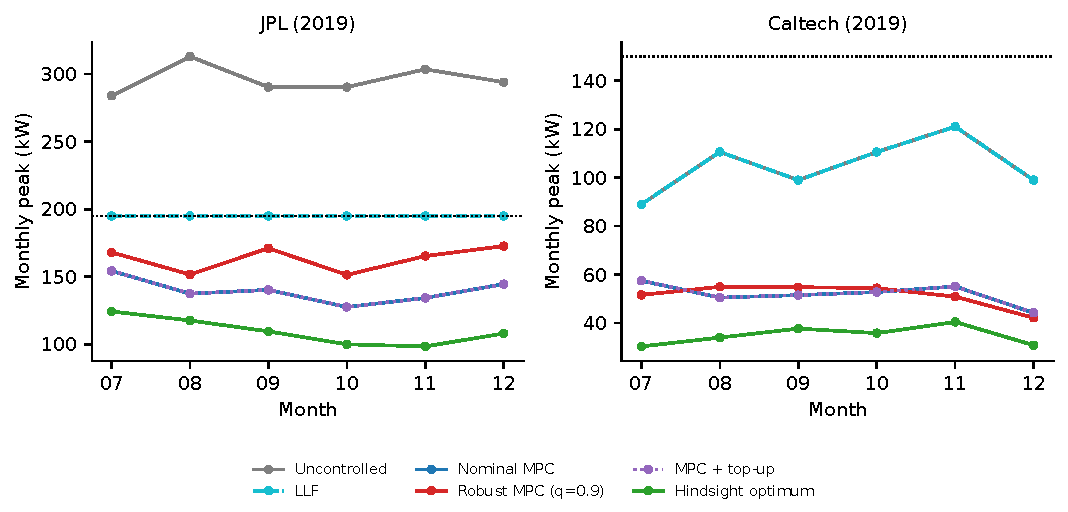
\includegraphics[width=0.9\textwidth]{figures/Fig7_monthly_peaks.pdf}
\caption{Monthly peak demand by policy. The dotted line is the site capacity. At Caltech the capacity never binds, so LLF (and EDF) coincide with uncontrolled charging and the uncontrolled line is hidden behind the LLF line; MPC + top-up has the same peak as nominal MPC by construction.}
\label{supp:peaks}
\end{figure}

\section{Load-duration curves}
Fig.~\ref{supp:ldc} shows the normalised load-duration curves underlying the grid-flexibility metrics of Section~6.2.

\begin{figure}[H]
\centering
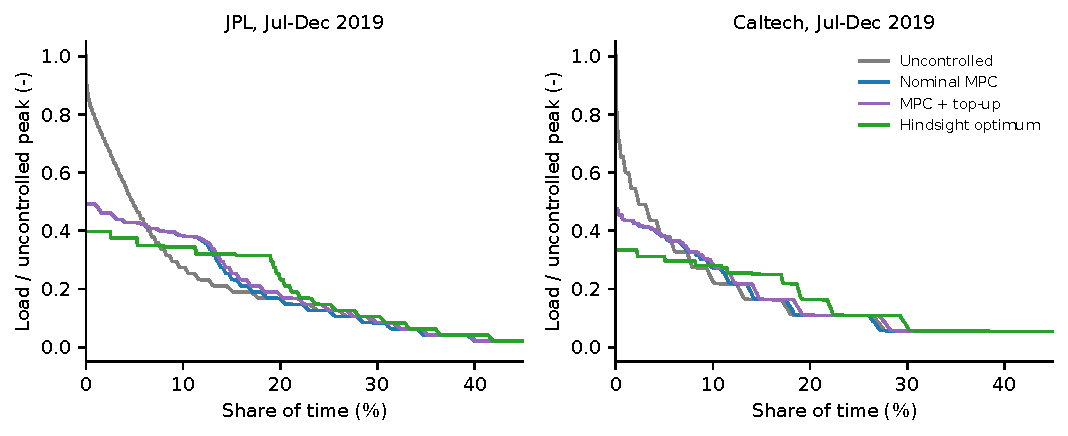
\includegraphics[width=0.9\textwidth]{figures/Fig11_load_duration.pdf}
\caption{Normalised load-duration curves (July--December 2019), load divided by the uncontrolled peak. Only the top 45\% of the time axis is shown; the remainder is near zero for all policies.}
\label{supp:ldc}
\end{figure}

\section{On-peak energy and solar coincidence}
Table~\ref{tab:solar} reports the on-peak energy share and the solar-coincidence metrics of Section~4.7 for the PV-unaware policies, and Fig.~\ref{supp:pv} compares the August weekday load profiles with the output of an energy-neutral clear-sky PV array. Flattening the morning spike moves charging towards midday. With a half-size array the gains are smaller but have the same sign; self-sufficiency is then 33--38\% for all policies because the array covers less of the load. Under TOU-EV-4 the same shift raises the share of energy in the 12--18\,h on-peak block and the time-of-use energy cost by about 5\% relative to uncontrolled charging.

\begin{table}[H]
\centering
\caption{On-peak energy and solar-coincidence metrics (July--December 2019).}
\label{tab:solar}
\footnotesize
\setlength{\tabcolsep}{1.5pt}
\begin{tabular*}{\textwidth}{@{\extracolsep{\fill}}llrrrr@{}}
\hline
Site & Policy & \makecell[c]{On-peak\\energy (\%)} & \makecell[c]{PV self-\\suff. (\%)} & \makecell[c]{PV util.\\(\%)} & \makecell[c]{PV self-suff.,\\half array (\%)} \\
\hline
JPL & Uncontrolled & 24.7 & 46.7\,{\scriptsize(45.1--48.9)} & 46.7 & 32.7 \\
JPL & LLF & 24.9 & 47.4\,{\scriptsize(46.2--49.2)} & 47.4 & 32.8 \\
JPL & Nominal MPC & 25.5 & 52.6\,{\scriptsize(49.5--56.2)} & 50.5 & 34.0 \\
JPL & Robust MPC, $q$=0.9 & 24.5 & 48.5\,{\scriptsize(47.0--49.8)} & 46.7 & 32.6 \\
JPL & MPC + top-up & 28.3 & 53.4\,{\scriptsize(51.0--56.7)} & 53.3 & 33.5 \\
JPL & MPC + top-up, $q$=0.7 & 36.4 & 60.5\,{\scriptsize(57.2--64.9)} & 59.5 & 34.9 \\
JPL & Hindsight opt. & 31.4 & 55.6\,{\scriptsize(50.5--62.0)} & 55.6 & 33.3 \\
\hline
Caltech & Uncontrolled & 26.9 & 56.1\,{\scriptsize(51.9--59.9)} & 56.1 & 35.2 \\
Caltech & LLF & 26.9 & 56.1\,{\scriptsize(51.9--59.9)} & 56.1 & 35.2 \\
Caltech & Nominal MPC & 31.6 & 59.4\,{\scriptsize(55.0--63.5)} & 57.2 & 36.3 \\
Caltech & Robust MPC, $q$=0.9 & 33.6 & 60.7\,{\scriptsize(56.6--65.5)} & 56.8 & 36.6 \\
Caltech & MPC + top-up & 33.9 & 59.7\,{\scriptsize(54.8--63.9)} & 59.2 & 36.0 \\
Caltech & MPC + top-up, $q$=0.7 & 38.7 & 64.3\,{\scriptsize(56.9--69.8)} & 62.4 & 37.7 \\
Caltech & Hindsight opt. & 31.4 & 59.2\,{\scriptsize(55.3--64.0)} & 59.2 & 34.9 \\
\hline
\end{tabular*}
\par\smallskip\parbox{\textwidth}{\scriptsize On-peak energy is the share delivered in the 12--18\,h weekday block. PV self-sufficiency is the share of EV energy coincident with an energy-neutral clear-sky PV array (monthly range in parentheses); utilisation is the share of PV output absorbed by EVs.}
\end{table}


\begin{figure}[H]
\centering
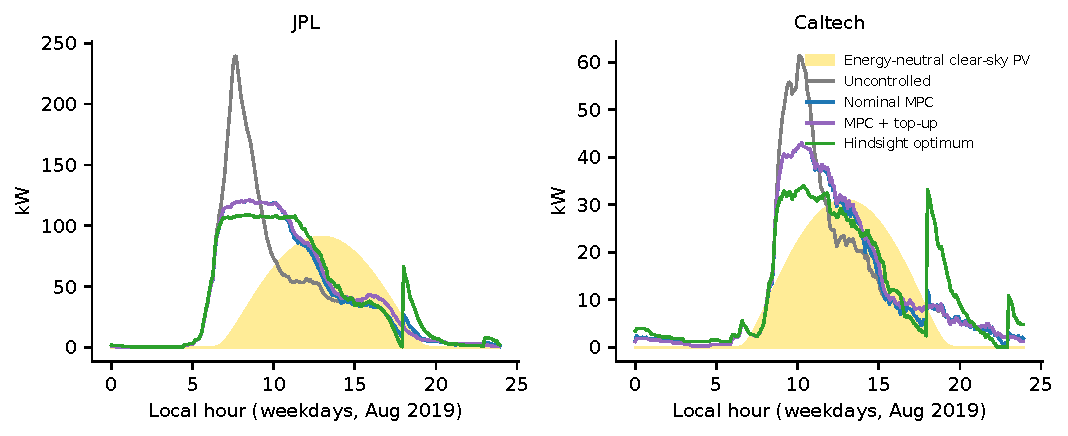
\includegraphics[width=0.9\textwidth]{figures/Fig12_pv_coincidence.pdf}
\caption{Mean weekday load profiles in August 2019 against the output of an energy-neutral clear-sky PV array (pvlib, Ineichen model).}
\label{supp:pv}
\end{figure}

\section{Calibrated uncertainty sets}
Fig.~\ref{supp:sets} shows the calibrated deadline shifts $\underline{\Delta d}=Q_{1-q}(\Delta d)$ and energy multipliers $\overline\rho=Q_q(\rho)$ for claimed sessions. At $q=0.5$ the deadlines move 0.5--1\,h later and declared energy is scaled to 0.52--0.65 of its declared value; at $q=0.9$ deadlines move 1.3--2.8\,h earlier while the energy multiplier only returns to about 1.0.

\begin{figure}[H]
\centering
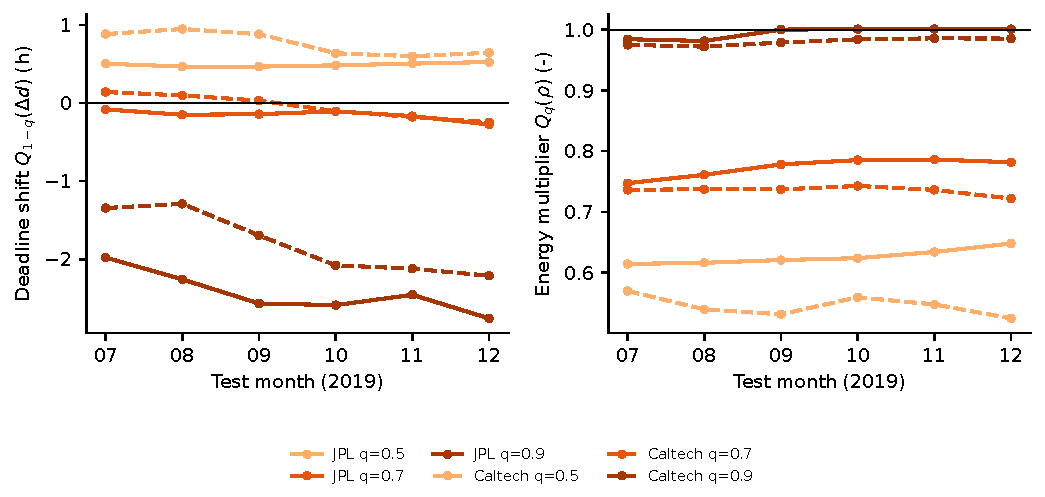
\includegraphics[width=0.9\textwidth]{figures/Fig8_calibrated_sets.pdf}
\caption{Calibrated deadline shifts and energy multipliers for claimed sessions by test month and protection level $q$.}
\label{supp:sets}
\end{figure}

\section{Sensitivity analysis}
Table~\ref{tab:sens} reports the sensitivity runs of Section~5.3 for August and November 2019 (nominal MPC, robust MPC at $q=0.9$ and, where the objective changes, the hindsight optimum).

\begin{table}[H]
\centering
\caption{Sensitivity analysis (means over August and November 2019).}
\label{tab:sens}
\footnotesize
\setlength{\tabcolsep}{1.5pt}
\begin{tabular*}{\textwidth}{@{\extracolsep{\fill}}lllrrr@{}}
\hline
Scenario & Site & Policy & \makecell[c]{Bill\\(USD)} & \makecell[c]{Peak\\(kW)} & \makecell[c]{Served\\(\%)} \\
\hline
Demand charge $\times$0 & JPL & Nominal MPC & 1,964\,{\scriptsize(1,439--2,490)} & 195.0 & 96.28 \\
Demand charge $\times$0 & JPL & Robust MPC, $q$=0.9 & 1,993\,{\scriptsize(1,440--2,547)} & 195.0 & 96.26 \\
Demand charge $\times$0 & JPL & Hindsight opt. & 2,023\,{\scriptsize(1,495--2,551)} & 195.0 & 100.00 \\
Demand charge $\times$0 & Caltech & Nominal MPC & 726\,{\scriptsize(513--938)} & 115.9 & 97.21 \\
Demand charge $\times$0 & Caltech & Robust MPC, $q$=0.9 & 723\,{\scriptsize(503--944)} & 115.9 & 95.38 \\
Demand charge $\times$0 & Caltech & Hindsight opt. & 708\,{\scriptsize(523--892)} & 115.9 & 100.00 \\
\hline
Demand charge $\times$2 & JPL & Nominal MPC & 6,275\,{\scriptsize(5,626--6,925)} & 135.9 & 96.10 \\
Demand charge $\times$2 & JPL & Robust MPC, $q$=0.9 & 5,270\,{\scriptsize(4,468--6,072)} & 99.0 & 91.17 \\
Demand charge $\times$2 & JPL & Hindsight opt. & 5,408\,{\scriptsize(4,613--6,204)} & 97.5 & 100.00 \\
Demand charge $\times$2 & Caltech & Nominal MPC & 2,226\,{\scriptsize(2,081--2,370)} & 46.5 & 95.19 \\
Demand charge $\times$2 & Caltech & Robust MPC, $q$=0.9 & 1,307\,{\scriptsize(1,176--1,439)} & 22.2 & 74.20 \\
Demand charge $\times$2 & Caltech & Hindsight opt. & 1,933\,{\scriptsize(1,785--2,082)} & 37.2 & 100.00 \\
\hline
Penalty 20\,USD/kWh & JPL & Nominal MPC & 4,148\,{\scriptsize(3,506--4,791)} & 134.8 & 96.06 \\
Penalty 20\,USD/kWh & JPL & Robust MPC, $q$=0.9 & 4,493\,{\scriptsize(4,013--4,974)} & 158.5 & 96.24 \\
Penalty 20\,USD/kWh & JPL & Hindsight opt. & 3,870\,{\scriptsize(3,086--4,655)} & 108.0 & 100.00 \\
Penalty 20\,USD/kWh & Caltech & Nominal MPC & 1,593\,{\scriptsize(1,387--1,798)} & 53.5 & 96.55 \\
Penalty 20\,USD/kWh & Caltech & Robust MPC, $q$=0.9 & 1,667\,{\scriptsize(1,482--1,852)} & 59.6 & 94.88 \\
Penalty 20\,USD/kWh & Caltech & Hindsight opt. & 1,356\,{\scriptsize(1,158--1,554)} & 37.2 & 100.00 \\
\hline
30-day window & JPL & Nominal MPC & 4,168\,{\scriptsize(3,542--4,793)} & 135.9 & 96.09 \\
30-day window & JPL & Robust MPC, $q$=0.9 & 4,485\,{\scriptsize(3,992--4,977)} & 158.4 & 96.06 \\
30-day window & Caltech & Nominal MPC & 1,582\,{\scriptsize(1,366--1,798)} & 52.8 & 96.45 \\
30-day window & Caltech & Robust MPC, $q$=0.9 & 1,557\,{\scriptsize(1,285--1,829)} & 52.2 & 94.18 \\
\hline
90-day window & JPL & Nominal MPC & 4,167\,{\scriptsize(3,542--4,792)} & 135.9 & 96.09 \\
90-day window & JPL & Robust MPC, $q$=0.9 & 4,503\,{\scriptsize(4,032--4,975)} & 159.2 & 96.22 \\
90-day window & Caltech & Nominal MPC & 1,569\,{\scriptsize(1,341--1,797)} & 52.0 & 96.41 \\
90-day window & Caltech & Robust MPC, $q$=0.9 & 1,564\,{\scriptsize(1,285--1,843)} & 52.7 & 94.09 \\
\hline
\end{tabular*}
\par\smallskip\parbox{\textwidth}{\scriptsize The range of the two months is shown in parentheses.}
\end{table}


\section{Robustness of the top-up rule}
Table~\ref{tab:topuprob} reports the top-up robustness runs of Section~6.10: the base case, site capacity scaled to 75\% and 50\%, twice the demand charge, 30- and 90-day calibration windows and a shortfall penalty of 20\,USD/kWh (four times the base value), each on August and November 2019 and on the held-out July and August 2021. Across all 56 scenario--site--month runs, the MPC + top-up peak equals the nominal MPC peak except in one month, where it is 1.8\,kW lower.

\begin{table}[H]
\centering
\caption{Robustness of the top-up rule. Means over August and November 2019 and over the held-out months July and August 2021. Served: energy served (\%) by nominal MPC (Nom.) and MPC + top-up (Top.); Full: vehicles fully served by MPC + top-up (\%); Peak red.\ and Saving: reduction of the monthly peak and of the bill of MPC + top-up relative to uncontrolled charging (\%). Site capacity scales the 195\,kW (JPL) and 150\,kW (Caltech) limits.}
\label{tab:topuprob}
\footnotesize
\setlength{\tabcolsep}{1.5pt}
\begin{tabular*}{\textwidth}{@{\extracolsep{\fill}}llrrrrrrrrrr@{}}
\hline
 & & \multicolumn{5}{c}{2019 (Aug, Nov)} & \multicolumn{5}{c}{2021 held out (Jul, Aug)} \\
Site & Scenario & Nom. & Top. & Full & \makecell[r]{Peak\\red.} & Saving & Nom. & Top. & Full & \makecell[r]{Peak\\red.} & Saving \\
\hline
JPL & Base case & 96.1 & 99.8 & 98.6 & 56 & 37 & 91.0 & 98.6 & 96.3 & 42 & 24 \\
 & Capacity $\times$0.75 & 96.1 & 99.8 & 98.7 & 56 & 37 & 91.0 & 98.6 & 96.1 & 43 & 25 \\
 & Capacity $\times$0.5 & 94.1 & 97.1 & 90.9 & 68 & 43 & 91.0 & 98.6 & 96.0 & 42 & 24 \\
 & Demand charge $\times$2 & 96.1 & 99.8 & 98.7 & 56 & 45 & 90.0 & 97.3 & 93.1 & 49 & 37 \\
 & 30-day calibration & 96.1 & 99.8 & 98.8 & 56 & 37 & 91.5 & 98.7 & 96.0 & 42 & 25 \\
 & 90-day calibration & 96.1 & 99.8 & 98.5 & 56 & 37 & 91.0 & 98.7 & 96.3 & 42 & 24 \\
 & Penalty $\times$4 & 96.1 & 99.7 & 98.7 & 56 & 37 & 91.0 & 98.6 & 96.1 & 42 & 24 \\
\hline
Caltech & Base case & 96.5 & 99.1 & 95.3 & 54 & 37 & 83.7 & 97.1 & 95.0 & 53 & 34 \\
 & Capacity $\times$0.75 & 96.5 & 99.1 & 95.4 & 54 & 37 & 83.7 & 97.1 & 95.0 & 53 & 34 \\
 & Capacity $\times$0.5 & 96.5 & 99.1 & 95.3 & 55 & 37 & 83.7 & 97.1 & 95.0 & 53 & 34 \\
 & Demand charge $\times$2 & 95.2 & 97.6 & 92.6 & 60 & 48 & 83.0 & 95.6 & 93.4 & 54 & 43 \\
 & 30-day calibration & 96.5 & 99.0 & 95.5 & 55 & 37 & 83.7 & 97.1 & 95.1 & 53 & 34 \\
 & 90-day calibration & 96.4 & 99.1 & 95.4 & 55 & 37 & 83.7 & 97.1 & 94.9 & 53 & 34 \\
 & Penalty $\times$4 & 96.5 & 99.2 & 95.8 & 54 & 36 & 83.8 & 97.3 & 95.3 & 52 & 34 \\
\hline
\end{tabular*}
\end{table}


\section{Higher driver demand}
Service in the main article is measured against the energy each vehicle received in the recorded sessions, which the ACN's own controller may have truncated. Table~\ref{tab:demandscale} therefore raises every session's energy need to $\alpha=1.1$ and $1.25$ times its recorded energy, capped at $\bar r_i$ times its plugged-in duration so that the need remains deliverable; sessions that already charged at their maximum rate cannot grow, so total demand rises by 8--10\% and 18--23\%. Declarations are unchanged, and the training windows used for calibration are scaled in the same way. Nominal MPC falls to 81--95\% served, MPC + top-up serves 96.0--99.5\%, never with a higher peak than nominal MPC, and the hindsight optimum serves at least 99.7\%.

\begin{table}[H]
\centering
\caption{Sensitivity to higher driver demand. Each session's energy need is raised to $\alpha$ times its historically delivered energy, capped at what its estimated maximum rate can deliver while plugged in; declarations are unchanged. Means over August and November 2019 and over the held-out July and August 2021. $\Delta E$: resulting increase in total demand (\%). Served: energy served (\%) by nominal MPC (Nom.), MPC + top-up (Top.) and the hindsight optimum (Opt.); Full: vehicles fully served by MPC + top-up (\%); Peak red.\ and Saving: peak and bill reduction of MPC + top-up relative to uncontrolled charging (\%).}
\label{tab:demandscale}
\scriptsize
\setlength{\tabcolsep}{1.5pt}
\begin{tabular*}{\textwidth}{@{\extracolsep{\fill}}llrrrrrrrrrrrrrr@{}}
\hline
 & & \multicolumn{7}{c}{2019 (Aug, Nov)} & \multicolumn{7}{c}{2021 held out (Jul, Aug)} \\
Site & $\alpha$ & $\Delta E$ & Nom. & Top. & Full & Opt. & \makecell[r]{Peak\\red.} & Saving & $\Delta E$ & Nom. & Top. & Full & Opt. & \makecell[r]{Peak\\red.} & Saving \\
\hline
JPL & 1.00 & +0 & 96.1 & 99.8 & 98.6 & 100.0 & 56 & 37 & +0 & 91.0 & 98.6 & 96.3 & 100.0 & 42 & 24 \\
 & 1.10 & +10 & 94.0 & 99.5 & 97.4 & 100.0 & 57 & 36 & +10 & 89.2 & 98.1 & 94.0 & 100.0 & 43 & 24 \\
 & 1.25 & +23 & 90.9 & 98.9 & 94.9 & 100.0 & 56 & 33 & +23 & 86.7 & 97.2 & 91.0 & 100.0 & 44 & 24 \\
\hline
Caltech & 1.00 & +0 & 96.5 & 99.1 & 95.3 & 100.0 & 54 & 37 & +0 & 83.7 & 97.1 & 95.0 & 99.9 & 53 & 34 \\
 & 1.10 & +9 & 94.5 & 98.6 & 93.4 & 100.0 & 60 & 41 & +8 & 82.7 & 96.6 & 94.1 & 99.9 & 53 & 34 \\
 & 1.25 & +22 & 91.4 & 97.4 & 90.9 & 100.0 & 61 & 41 & +18 & 81.0 & 96.0 & 92.4 & 99.7 & 56 & 35 \\
\hline
\end{tabular*}
\end{table}


\section{Tariff archetypes}
Table~\ref{tab:arch} compares TOU-EV-4 with the two stylised archetypes of Section~4.10, all with the same demand charge. The evening-peak TOU keeps the TOU-EV-4 price levels with the on-peak block at 16--21\,h on weekdays and mid-peak prices at 8--16\,h and 21--23\,h; the flat price is the monthly time-weighted mean of the TOU-EV-4 energy price.

\begin{table}[H]
\centering
\caption{Tariff archetypes, all with the 15.51\,USD/kW-month demand charge (means over August and November 2019).}
\label{tab:arch}
\footnotesize
\setlength{\tabcolsep}{1.5pt}
\begin{tabular*}{\textwidth}{@{\extracolsep{\fill}}llrrrrrr@{}}
\hline
Site & Energy price & \makecell[c]{Bill, unc.\\(USD)} & \makecell[c]{Bill, top-\\up (USD)} & \makecell[c]{Saving\\(\%)} & \makecell[c]{Energy\\cost (\%)} & \makecell[c]{Peak\\red. (\%)} & \makecell[c]{Served\\(\%)} \\
\hline
JPL & TOU-EV-4 & 6,853 & 4,305 & 37.2 & +6.1 & 55.9 & 99.8 \\
JPL & Evening TOU & 6,547 & 3,920 & 40.1 & +2.6 & 55.9 & 99.8 \\
JPL & Flat & 6,599 & 3,922 & 40.6 & -0.2 & 55.9 & 99.8 \\
\hline
Caltech & TOU-EV-4 & 2,553 & 1,616 & 36.7 & +5.4 & 54.4 & 99.1 \\
Caltech & Evening TOU & 2,443 & 1,461 & 40.2 & -0.7 & 54.4 & 99.0 \\
Caltech & Flat & 2,412 & 1,429 & 40.7 & -0.9 & 54.4 & 99.1 \\
\hline
\end{tabular*}
\par\smallskip\parbox{\textwidth}{\scriptsize Energy cost change is MPC + top-up relative to uncontrolled charging. The evening-peak and flat-price archetypes are stylised (Section 4.10).}
\end{table}


\bibliographystyle{elsarticle-num}
\bibliography{references}
\end{document}
